\section{Ablation Studies}
\label{sec:ablation}
All ablations use the low setting ($B{=}64$, $K_{\mathrm{eff}}\in[2,10]$) and the all-classes setting on the eleven datasets with CLIP ViT-B/16; grey entries are placeholders.

\paragraph{Components.}
\Cref{tab:components} adds the components one at a time. The presence model alone already removes part of the collapse, the anchor term removes the rest, and the graph coupling adds the margin that distinguishes \method from anchor-only methods; the inherited sample graph matters mainly in the all-classes setting, and empirical Bayes matches the fixed strengths without tuning.

\begin{table}[t]
  \centering\footnotesize
  \caption{\textbf{Component ablation}, top-1 accuracy (\%). $\pi$: presence; $\alpha$: anchor; $\lambda$: graph coupling; EB: empirical Bayes; $W_s$: sample graph.}
  \label{tab:components}
  \begin{tabular}{ccccc@{\hskip 10pt}cc}
    \toprule
    $\pi$ & $\alpha$ & $\lambda$ & EB & $W_s$ & Low ($B{=}64$) & All\\
    \midrule
    \multicolumn{5}{c}{zero-shot} & 65.2 & 65.2\\
    -- & -- & -- & -- & \checkmark & \ph{43.3} & \ph{70.3}\\
    \checkmark & -- & -- & -- & \checkmark & \ph{55.8} & \ph{70.3}\\
    -- & \checkmark & -- & -- & \checkmark & \ph{69.1} & \ph{69.9}\\
    \checkmark & \checkmark & -- & -- & \checkmark & \ph{69.6} & \ph{69.9}\\
    -- & \checkmark & \checkmark & -- & \checkmark & \ph{70.2} & \ph{70.2}\\
    \checkmark & \checkmark & \checkmark & -- & -- & \ph{70.4} & \ph{68.7}\\
    \checkmark & \checkmark & \checkmark & -- & \checkmark & \ph{70.7} & \ph{70.2}\\
    \checkmark & \checkmark & \checkmark & \checkmark & \checkmark & \ph{\textbf{70.8}} & \ph{70.2}\\
    \bottomrule
  \end{tabular}
\end{table}

\paragraph{Prior and graph.}
\Cref{tab:prior} and \cref{fig:sens} vary $\alpha$, $\lambda$ and the number of neighbours $m$, and replace the text kNN graph by a complete graph and by a degree-matched random graph. The random-graph row separates pooling from pooling \emph{along semantics}: a random graph performing as well as $L_T$ would refute Hypothesis~\ref{hyp:smooth}. Accuracy is flat over an order of magnitude of $\lambda$ and $m$, and the complete graph (a single shift) recovers only part of the gain.

\begin{table}[t]
  \centering
  \caption{\textbf{Prior and graph ablation}, low setting. Default: $\alpha{=}1$, $\lambda{=}4$, $m{=}5$, $\rho{=}0.05$.}
  \label{tab:prior}
  \footnotesize\setlength{\tabcolsep}{2.5pt}
  \begin{tabular}{@{}lcccccc@{}}
    \toprule
    $\alpha$ & 0 & 0.25 & 1 & 4 & 16 & \\
    acc. & \ph{69.0} & \ph{70.2} & \ph{\textbf{70.7}} & \ph{70.4} & \ph{69.6} & \\
    \midrule
    $\lambda$ & 0 & 1 & 4 & 16 & 64 & $\infty$\\
    acc. & \ph{69.1} & \ph{70.1} & \ph{\textbf{70.7}} & \ph{70.5} & \ph{69.9} & \ph{68.8}\\
    \midrule
    graph & $m{=}3$ & $m{=}5$ & $m{=}10$ & compl. & rand. & \\
    acc. & \ph{70.4} & \ph{\textbf{70.7}} & \ph{70.5} & \ph{68.8} & \ph{69.2} & \\
    \bottomrule
  \end{tabular}
\end{table}

\begin{figure}[t]
  \centering
  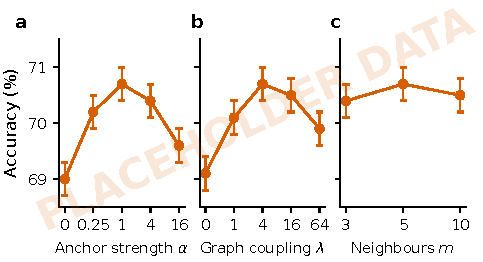
\includegraphics[width=\linewidth]{figures/plot_sensitivity.pdf}
  \caption{\textbf{Sensitivity} to the prior strengths and graph size (low setting, mean $\pm$ std over tasks). Placeholder data.}
  \label{fig:sens}
\end{figure}

\paragraph{Likelihood, optimisation and cost.}
A supplementary table compares the shared diagonal covariance with isotropic and per-class variants, prototype re-projection, the pseudo-count $c$, the temperature $\kappa$ and the number of iterations, and lists asymptotic and measured cost; with conjugate gradients \method adds one sparse $K\times K$ solve per dimension block to StatA, of the same order as one E-step, and processes a batch of 64 ImageNet images in \ph{9} ms on one GPU against \ph{7} ms for StatA.
